Performing row operations
on the matrix
\begin{align*}  
\myvec{
    3 &1&-2 \\
     p&2&-3\\
     2&-1&-3
}
\xrightarrow[R_3=3R_3-2R_1]{R_2=3R_2-pR_1}&\myvec{
    3&1&-2\\
     $0$&6-p&-9+2p\\
     0&-5&-5}\\
 \xrightarrow{R_3=R_3(6-p)+5R_2}&\myvec{
    3&1&-2\\
     0&6-p&-9+2p\\
     0&0&-75+15p}
     \\
  \implies 
    p=5
\end{align*}
Substituting this value in the above, we obtain
\begin{align}
\myvec{
    3&1&-2\\
     0&1&1\\
     0&0&0}
\end{align}
yielding
\begin{align}
	\vec{x} = \myvec{-1 \\ 1}
\end{align}
as the point of intersection.
    See \figref{fig:11.10.4.9}.
\begin{figure}[H]
    \centering
    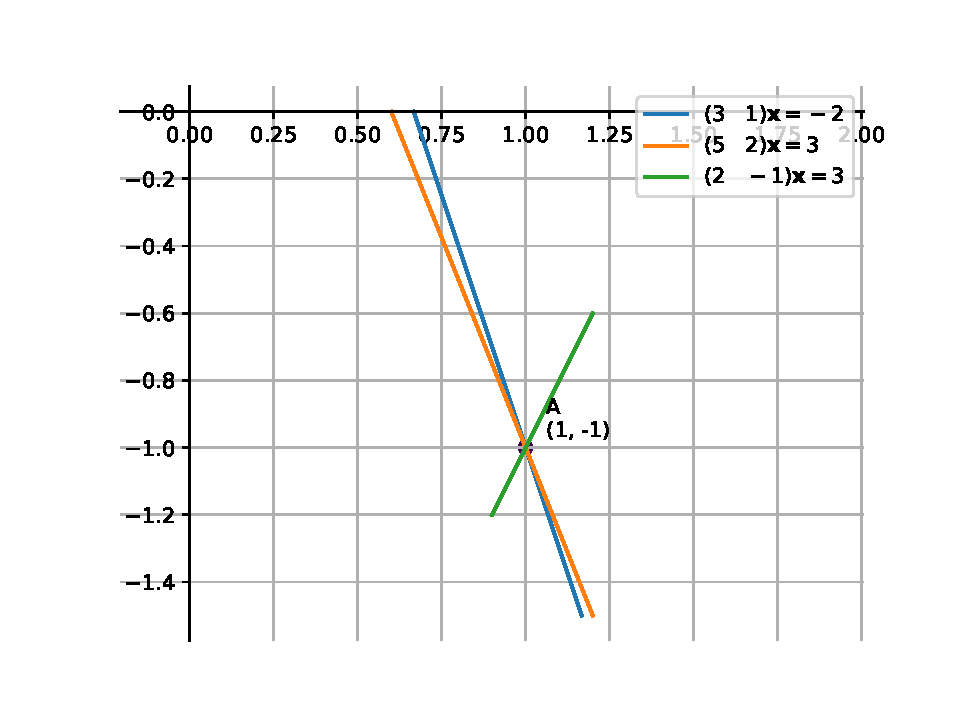
\includegraphics[width=0.75\columnwidth]{chapters/11/10/4/9/figs/fig.pdf}
    \caption{}
    \label{fig:11.10.4.9}
\end{figure}

